%\todofilebegin{040\_evaluation\_validation.tex}
%%%%%%%%%%%%%%%%%%%%%%%%%%%%%%%%%%%%%%%%%%%%%%%%%%%%%%%%%%%%%%%%%%%%%%%%%%%%%%
%%%%%%%%%%%%%%%%%%%%%%%%%%%%%%%%%%%%%%%%%%%%%%%%%%%%%%%%%%%%%%%%%%%%%%%%%%%%%%
%%%%%%%%%%%%%%%%%%%%%%%%%%%%%%%%%%%%%%%%%%%%%%%%%%%%%%%%%%%%%%%%%%%%%%%%%%%%%%

\section{Evaluation and Validation}

SOSflow is a large, complex, and completely new tool framework. The
core library components comprise more than 12,000 lines of original
C99 code. SOSflow's code base has \textit{not} been systematically
optimized for this pre-release research work -- since it is an open
source project, volunteers are always welcome! It is likely that the
observed performance of SOSflow will dramatically improve with several
iterations of focused overhead and latency refactoring. Many of the
behavioral characteristics of SOSflow are the product of its internal
parameters and the configuration of its runtime deployment, rather
than products of its data model and algorithms. The exploration of
optimal settings in that combined parameter space is left for future
work: For now the effort was made to select reasonable default SOSflow
configuration parameters and typical/non-priviledged cluster
queues and topologies.

SOSflow as a tool is \textit{production capable} for the purpose of
validating the SOS workflow performance model. As we demonstrate, even
the current un-optimized code is able to scale out to reasonable
allocation sizes and handle relatively impressive varieties,
quantities, and rates of data flow. Because of the lack of focused
tuning to its internal mechanics and the general novelty of the
architecture, the results and figures presented here should be
considered the \textit{worst-case scenario} for the performance of
SOSflow itself, now and for the future.

%-----------------------------------------------------------------------------
\subsection{Testing Platform and SOS Configurations}

Single node tests of SOSflow were performed by launching the
sosd(listener) daemon along with an sosd(db) instance as background MPI tasks.
The demo\_app tool was then also launched as an MPI task with varying parameters
to explore the capabilities of the sosd daemons.

Tests run on the ACISS platform at the University of Oregon were
deployed with the Torque job scheduler as MPI applications at scales
ranging from 3 to 24 nodes, serving 10 demo\_app processes per
node. These runs were tuned as stress tests to make ensure the daemons
could operate under reasonable but heavy loads.

Real-world use case experiments were conducted on the Cori
supercomputer at The National Energy Research Scientific Computing
Center NERSC. An SOSflow-enabled variant of the Tuning and Analysis
Utilities program (TAUflow) was created as a part of the SOSflow
development work. On Cori, TAUflow was used to instrument the
Livermore Unstructured Lagrangian Explicit Shock Hydrodynamics
(LULESH) code. During the execution of LULESH, a thread would
periodically awaken and submit all of TAU's observed performance
metrics into the SOSflow system. SOSflow's presence and activity in
situ effected just over 1\% percent increase in the execution time of
LULESH on Cori, for scales of 8 to 512 client processes.  See
figure~\ref{cori_results} on page~\pageref{cori_results}.


%-----------------------------------------------------------------------------
\subsection{Latency}

When messages are received over the socket by the sosd(listener)
daemon, they are placed in an asynchronous task queue rather than
being handled immediately. This allows the socket reading loop to
immediately return to listening for another connection.  There are
three threads running inside the daemon that resolve messages:
local\_sync, node\_sync, and db\_sync.  The local\_sync thread picks up
the incoming messages from the queue first, unpacks the message and
updates the in-memory data structures. The local\_sync message handler
concludes by creating appropriate tasks in the db\_sync queue to
schedule new values for storage, and then places the original message
in the node\_sync queue for transmission to a sosd(db) aggregator.

The latency figures shown here reveal how long a value is floating in
the asynchronous queues of the daemon before being stored in the
database. Practically speaking this indicates how long it takes after
a value is published before it is available for searching by an
analytics module.  Latency in this context \textit{not} the time cost
of calling SOSflow functions, a blocking API call that messages a
daemon over the socket is nearly constant time regardless of daemon
load.

When a value is inserted into the database the time\_recv field is set,
the time\_pack and time\_sent fields having already been filled by the
original source of the value.  Latency is calculated by subtracting
the time\_sent from the time\_recv figures. When a message is migrated
from a sosd(listener) instance to a sosd(db) aggregate daemon, it is
packed up together with many other messages and sent over MPI.  On
receipt by an sosd(db) role, those composite messages are broken apart
and immediately serviced, causing the db\_sync queue to grow rapidly in
brief bursts as large quantities of data can be arriving all at once.
It is expected that the upper bound on latency for sosd(db) roles will
be higher than the in situ databases.

The asynchronous queues have thread-sequential FIFO ordering, but
because the MPI messages are queued up based on their arrival time,
and a batch is handled competely before the next is processed, there
is no real-time interleaving of database value injections, they are
injected in batches. This creates the sawtooth pattern in
figures~\ref{aciss_lat_3_agg} and \ref{aciss_lat_24_agg}, as the latency for values in the
batches near the bottom of the pile of MPI messages consistently
increases until their batch is injected.

\begin{figure*}[!t]
\centering
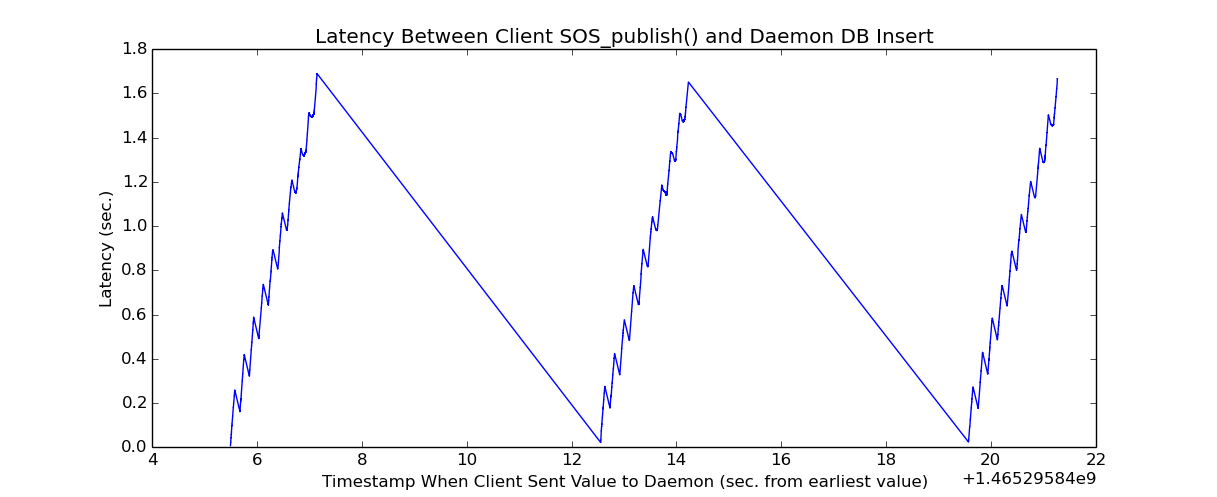
\includegraphics[width=5in]{images/aciss_latency_3_situ.png}
\caption{In Situ Latency (3 Nodes, 30 Applications)}
\label{aciss_lat_3_situ}
\end{figure*}

\begin{figure*}[!t]
\centering
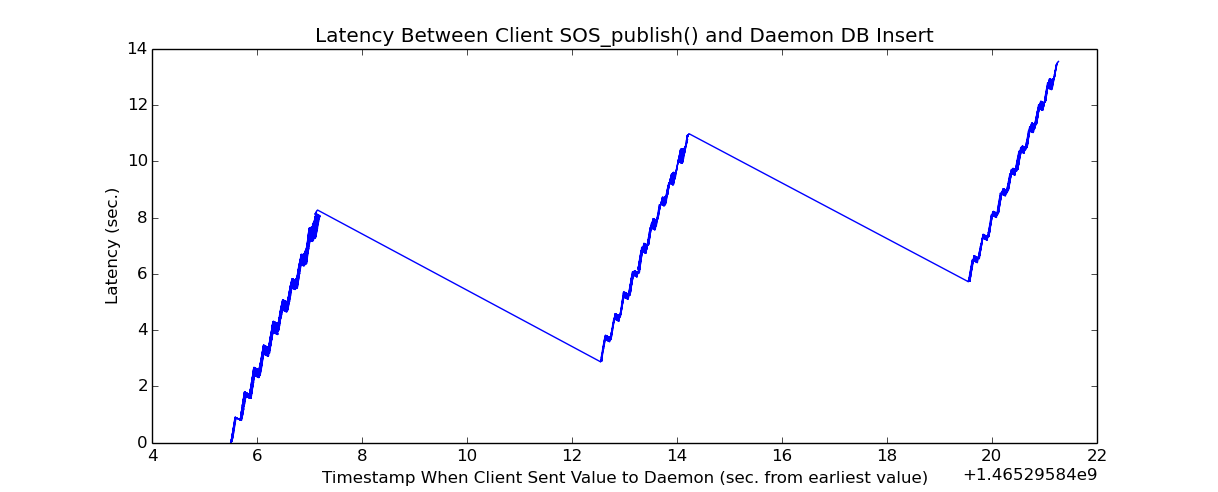
\includegraphics[width=5in]{images/aciss_latency_3_agg.png}
\caption{Aggregate sosd(db) Latency (3 Nodes, 30 Applications)}
\label{aciss_lat_3_agg}
\end{figure*}

\begin{figure*}[!t]
\centering
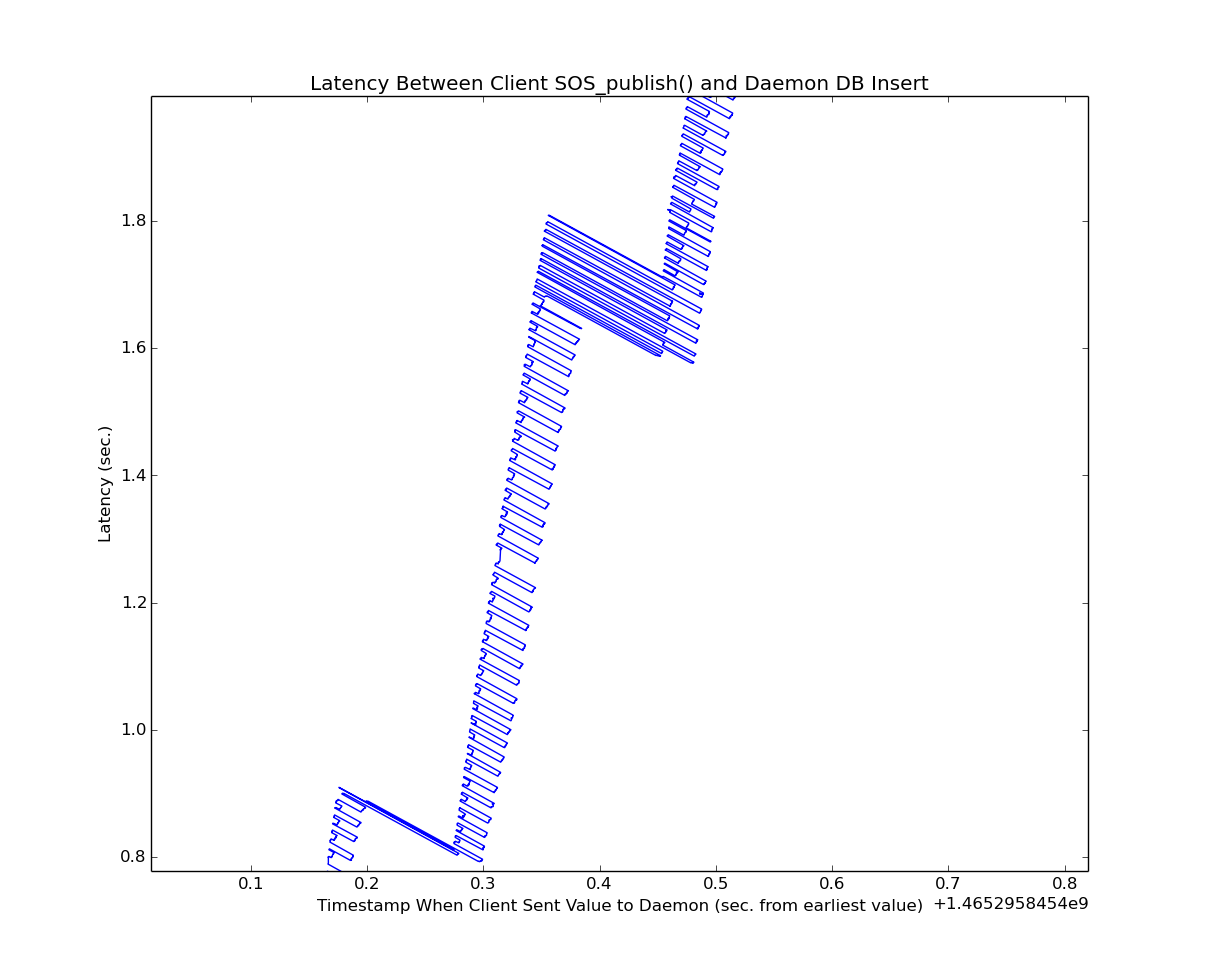
\includegraphics[width=5in]{images/aciss_latency_3_agg_zm.png}
\caption{Aggregate sosd(db) Detail (3 Nodes, 30 Applications)}
\label{aciss_lat_3_agg_detail}
\end{figure*}


\begin{figure*}[!t]
\centering
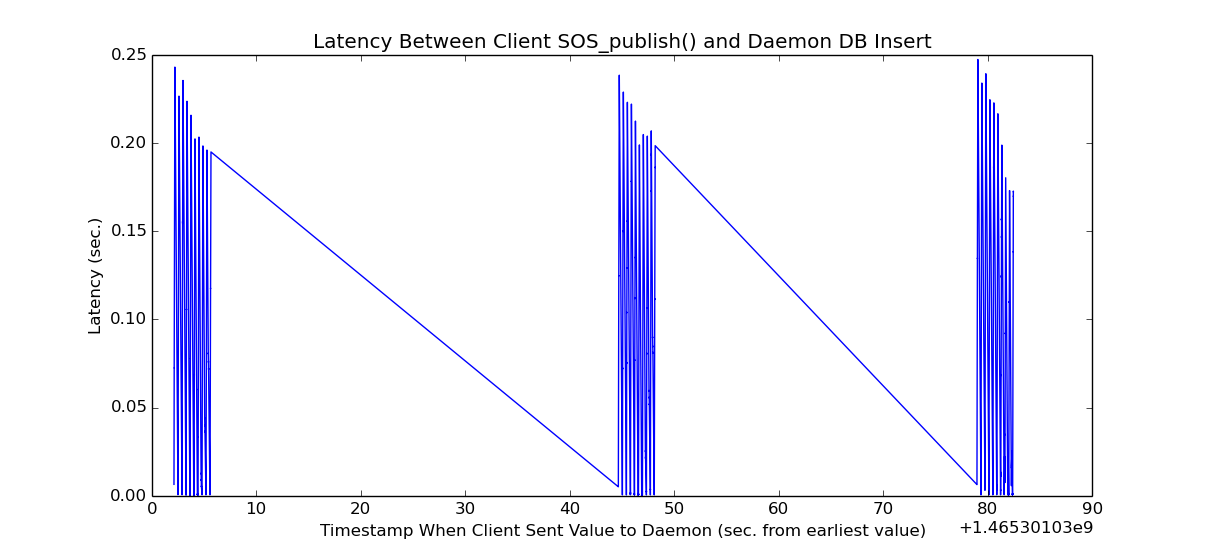
\includegraphics[width=5in]{images/aciss_latency_24_situ.png}
\caption{In Situ Latency (24 Nodes, 240 Applications)}
\label{aciss_lat_24_agg}
\end{figure*}


\begin{figure*}[!t]
\centering
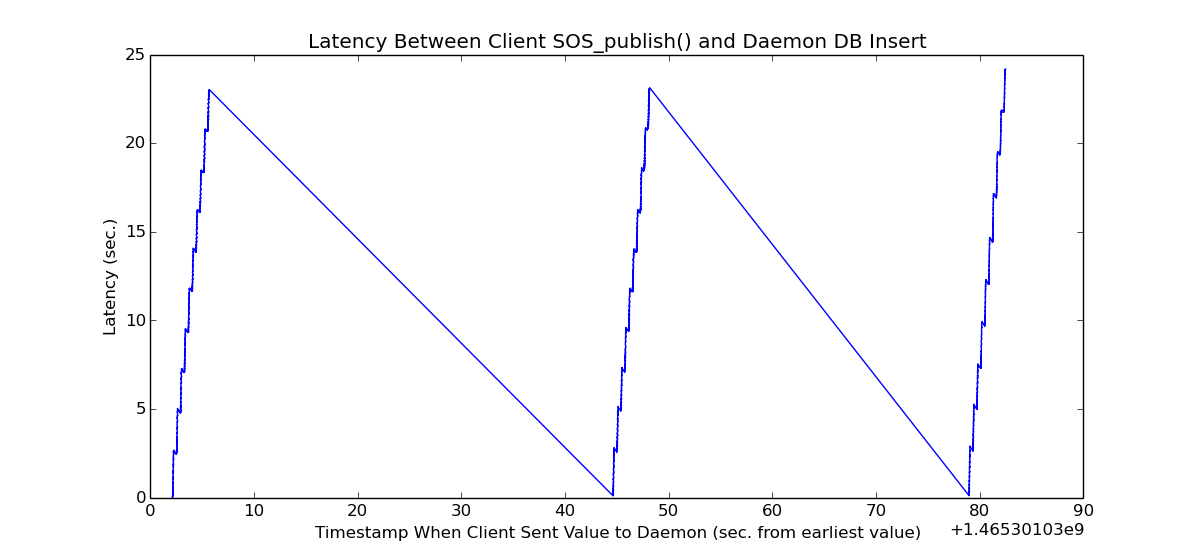
\includegraphics[width=5in]{images/aciss_latency_24_agg.png}
\caption{Aggregate sosd(db) Latency (24 Nodes, 240 Applications)}
\label{aciss_lat_24_agg}
\end{figure*}



%-----------------------------------------------------------------------------
\subsection{Scalability}


\begin{figure*}[!t]
\centering
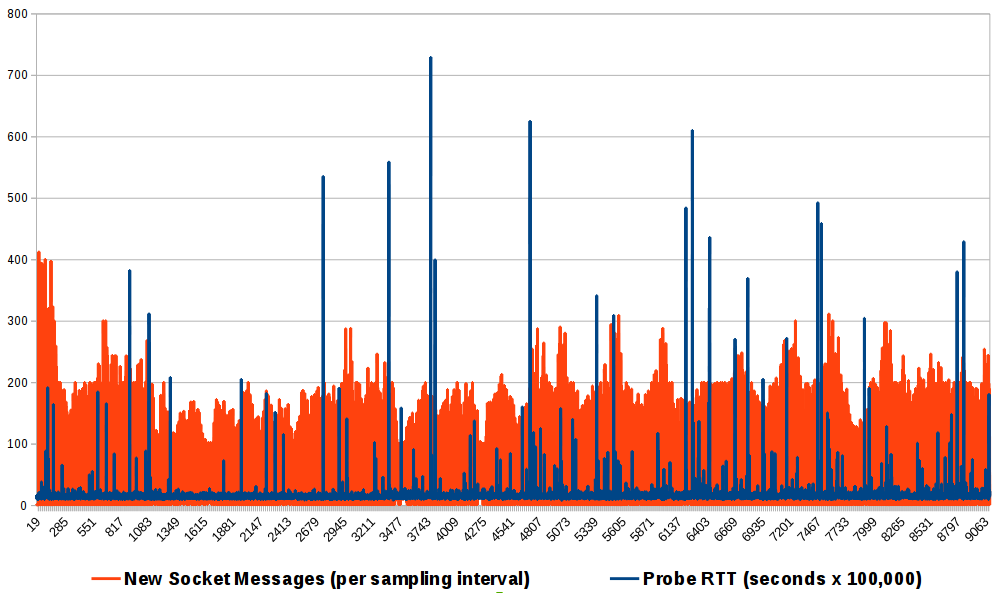
\includegraphics[width=5in]{images/icebox_api_cost_when_slam.png}
\caption{SOSflow Socket Communication Cost (~0.003sec)}
\label{sock_cost}
\end{figure*}


\begin{figure*}[!t]
\centering
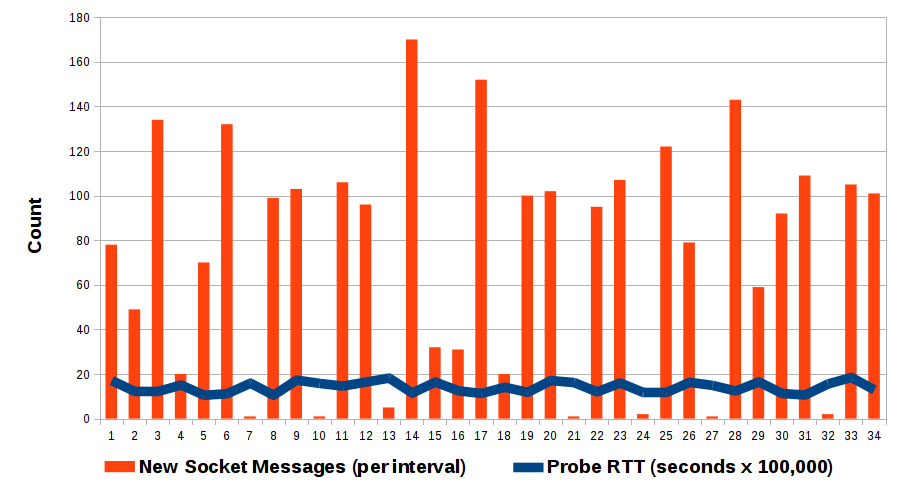
\includegraphics[width=5in]{images/icebox_api_cost_zoom.png}
\caption{SOSflow Socket Communication Cost, Detail}
\label{sock_cost_detail}
\end{figure*}


The data store used by SOS at this time is Sqlite3. It was chosen for
its simplicity and essential functionality, and because its license
is open. The configuration for these experiments has Sqlite3 creating
a file and writing to it, rather than representing the database only in
RAM -- though /dev/shm memory-mapped folders are used as the working
directory for the data store wherever possible. For reasonable rates of
data injection, Sqlite3 serves the project well, but at larger scales
it is expected that it will be replaced with a more robust data store.




%-----------------------------------------------------------------------------
\subsection{Overhead and Perturbation}

\begin{figure*}[!t]
\centering
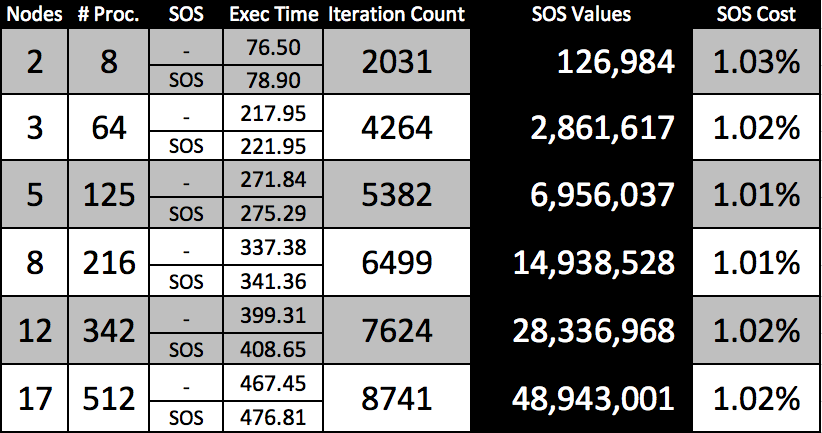
\includegraphics[width=5in]{images/cori_results.png}
\caption{Impact of SOSflow on LULESH Experiments}
\label{cori_results}
\end{figure*}


%\todofileend{040\_evaluation\_validation.tex}
